\documentclass[11pt,a4paper]{article}
\usepackage[margin=2.3cm]{geometry}
\usepackage{amsmath,amssymb}
\usepackage{booktabs}
\usepackage{graphicx}
\usepackage[font=small,labelfont=bf]{caption}
\usepackage{microtype}
\usepackage[hidelinks]{hyperref}
\newcommand{\NSessions}{8}
\newcommand{\NTrials}{5{,}141}
\newcommand{\NSamples}{1.6}
\newcommand{\NNogo}{19}
\newcommand{\AlignSD}{9}
\newcommand{\AlignSDmin}{6}
\newcommand{\AlignSDmax}{11}
\newcommand{\LagMed}{68}
\newcommand{\LagMin}{55}
\newcommand{\LagMax}{110}
\newcommand{\GainMin}{110}
\newcommand{\GainMax}{126}
\newcommand{\PreMAE}{0.9}
\newcommand{\PreMedAE}{0.22}
\newcommand{\PreRtwo}{0.992}
\newcommand{\PreTick}{80}
\newcommand{\PostMAE}{2.0}
\newcommand{\TzeroMAE}{30}
\newcommand{\TtwoMAE}{2.7}
\newcommand{\NTrialRtwo}{5{,}118}
\newcommand{\NFlat}{4}
\newcommand{\TrialRtwoMed}{0.96}
\newcommand{\TrialRtwoNine}{75}

\sloppy

\title{Decoding the on-screen stimulus position\\from wheel position and trial timing in the IBL task}
\author{Michael Schartner}
\date{18 November 2026}

\begin{document}
\maketitle

\begin{abstract}
In the IBL visual decision task, the mouse moves a Gabor patch across the screen by turning a wheel.
The stimulus position is not part of the standard ALF trials data. We ask whether it can be reconstructed
from the wheel position and the trial event times. As ground truth we use the position log written by the
task software (Bonsai), aligned to the photodiode. We tested \NSessions{} brain-wide map sessions (one per lab,
\NTrials{} trials). A closed-form model with no free gain recovers the stimulus azimuth to within
\PreMAE$^\circ$ mean absolute error ($R^2=\PreRtwo$) between stimulus onset and response. This model is
$x(t) = x_0 + G\,[w(t-\tau) - w(t_\mathrm{on}-\tau)]$, with $G=4^\circ/\mathrm{mm}\times 31\,\mathrm{mm}$ and a
display lag $\tau\approx\LagMed$\,ms. Its only unknown is the initial side $x_0=\pm35^\circ$. The side can be
inferred on answered trials (5{,}121 of 5{,}122) from the wheel direction at response together with the
outcome-specific stimulus-off delay. On no-go trials it cannot be inferred. Data-driven decoders given the wheel without the
event times reach only $\sim$\TzeroMAE$^\circ$ error.
\end{abstract}

\section{Task and stimulus mechanics}
In each trial a Gabor patch (contrast 0--100\%, $\sigma=7^\circ$) appears at azimuth $x_0=-35^\circ$ (left) or
$+35^\circ$ (right). From that moment the wheel controls the stimulus in closed loop: the azimuth changes by
$4^\circ$ per mm of wheel-surface displacement (task setting \texttt{STIM\_GAIN}). The response is registered
when the stimulus has moved $35^\circ$ from its start (\texttt{ALL\_THRESHOLDS}). A correct response brings the
stimulus to the centre ($0^\circ$). An error drives it to $\pm70^\circ$. The stimulus then stays on screen
$\approx$1\,s after correct feedback and $\approx$2\,s after error feedback (timeout). If the mouse makes no
response for 60\,s, the trial is a no-go, which counts as an error with almost no stimulus-off delay. All
sessions used here ran iblrig version 6 (6.2.5--6.5.3), and all used these settings.

\section{Data}
\paragraph{Sessions.} We took one session per lab from the IBL brain-wide map release
(\texttt{brainwidemap.bwm\_query}, 2023\_12 fixture), keeping the first session of each lab that had the raw
stimulus-position log. This gave \NSessions{} sessions from 8 labs (Table~\ref{tab:sessions}): \NTrials{} trials,
of which \NNogo{} were no-go, and \NSamples\,M evaluation samples.

\paragraph{Ground truth.} During each session Bonsai writes \texttt{raw\_behavior\_data/}\allowbreak\texttt{\_iblrig\_stimPositionScreen.raw.csv}.
Each row holds three columns: the contrast currently shown (0 when no stimulus is on screen), the stimulus
azimuth in degrees, and a Bonsai wall-clock timestamp. A row is written only when a value changes, so the log
is read as a zero-order hold. The azimuth changes in steps of $0.761^\circ$. This is exactly one step of the
1024-count rotary encoder, $2\pi/1024\,\mathrm{rad}\times 31\,\mathrm{mm}\times 4^\circ/\mathrm{mm}$, so the log
reflects the encoder count directly.

\paragraph{Wheel and trials.} We used the ALF objects \texttt{wheel} (\texttt{position} in radians,
\texttt{timestamps} in session time) and \texttt{trials} (\texttt{stimOn\_times}, \texttt{response\_times},
\texttt{feedback\_times}, \texttt{stimOff\_times}, \texttt{contrastLeft/Right}, \texttt{choice},
\texttt{feedbackType}), loaded with ONE. The wheel position at arbitrary times is obtained by linear interpolation.

\paragraph{Clock alignment.} We map the Bonsai wall clock to session time in two steps.
\begin{enumerate}
\item A coarse linear fit matches the per-trial wall-clock stamps in
\texttt{\_iblrig\_encoderTrialInfo.raw.ssv} to \texttt{trials.intervals[:,0]}.
\item Using the coarse fit, each Bonsai stimulus onset (the contrast column changing from 0 to $>0$; not
available for 0\% contrast trials) is matched to the nearest photodiode \texttt{stimOn\_times}. Matches that
deviate by more than 50\,ms from the median offset are discarded. A second linear fit is made on the remaining
pairs.
\end{enumerate}
Bonsai onsets precede the photodiode by $\approx$50--100\,ms. Aligning to the photodiode therefore puts every
logged position at the time it was actually displayed. The residual of the second fit had a standard deviation
of \AlignSDmin--\AlignSDmax\,ms (median \AlignSD\,ms), which is below one 60\,Hz frame.

\paragraph{Evaluation samples.} For each trial with finite event times we sample a 10\,ms grid from
\texttt{stimOn} to \texttt{stimOff}, the interval in which the stimulus is on screen. The ground truth at each
sample is the last logged azimuth at or before that time. Samples are grouped into three epochs:
stimOn--response and response--stimOff on answered trials, and all samples of no-go trials. No-go trials last
up to 60\,s, so pooling them with answered trials would let a handful of trials dominate.

\section{Models}
\subsection{Physics model}
Let $w(t)$ be the wheel angle in radians, $t_\mathrm{on}$ the photodiode stimulus onset and $t_\mathrm{resp}$
the response time. The predicted azimuth is
\begin{equation}
\hat x(t) = x_0 + G\,\bigl[w(\min(t-\tau,\ t_\mathrm{resp})) - w(t_\mathrm{on}-\tau)\bigr],
\qquad G = -4\,\tfrac{\circ}{\mathrm{mm}}\times 31\,\mathrm{mm} = -124^\circ/\mathrm{rad}.
\label{eq:physics}
\end{equation}
\begin{itemize}
\item \textbf{Gain.} The magnitude of $G$ is fixed by the task settings and the wheel radius; nothing is fitted.
The sign gives the convention: positive (counter-clockwise) wheel rotation in ALF moves the stimulus to
negative azimuth. The sign was estimated per session and was the same in all sessions.
\item \textbf{Display lag $\tau$.} What is on screen at time $t$ reflects the wheel as it was at $t-\tau$. This
lag combines encoder and Bonsai processing with the rendering pipeline. We fit $\tau$ per session by a grid
search (0--150\,ms in 5\,ms steps) that minimises the mean absolute error of Eq.~\ref{eq:physics} on
stimOn--response samples of answered trials, with the side known. This is the only fitted parameter, and it is
fitted in-sample.
\item \textbf{Freeze at response.} When the threshold is crossed, Bonsai stops moving the stimulus. The screen
catches up to the threshold crossing $\tau$ later, so the prediction holds $w(t_\mathrm{resp})$ for all
$t-\tau\ge t_\mathrm{resp}$.
\item \textbf{Reference.} Displacement is measured from $w(t_\mathrm{on}-\tau)$, the wheel state that
corresponds to the first displayed frame.
\end{itemize}
As a consistency check we also fitted an unconstrained gain by least squares at the fitted $\tau$. It gave
$|G_\mathrm{free}| = \GainMin$--$\GainMax^\circ$/rad, against the nominal 124 (Table~\ref{tab:sessions}). The
two lowest values come from the sessions with the largest alignment jitter, which is what one expects from
regression dilution caused by timing noise.

\subsection{Initial side \texorpdfstring{$x_0$}{x0}}
\begin{itemize}
\item \textbf{Side known:} $x_0=-35^\circ$ if \texttt{contrastLeft} is defined, and $+35^\circ$ otherwise.
\item \textbf{Side inferred from wheel and timing only:} the direction in which the stimulus moved at
response, $c=-\operatorname{sign}\bigl(G\,[w(t_\mathrm{resp})-w(t_\mathrm{on}-\tau)]\bigr)$, gives the side
the stimulus came from if the trial was correct. The outcome is read from the stimulus-off delay
$t_\mathrm{off}-t_\mathrm{fb}$, which clusters at $\approx$1.07\,s for correct, $\approx$2.07\,s for error and
$\approx$0.06\,s for no-go trials. We set $x_0=35c$ if the delay is below 1.5\,s, $x_0=-35c$ if it is above
1.5\,s, and $x_0=0$ if it is below 0.5\,s (no-go). This rule uses information from later in the trial, so it
is suitable for offline regressors but not for a causal, online estimate. Before the first movement the side
cannot be determined from the wheel.
\end{itemize}

\subsection{Data-driven baselines}
To ask how much the event times contribute, we trained gradient-boosted regression trees
(\texttt{sklearn} \texttt{HistGradientBoostingRegressor}, 300 iterations, learning rate 0.1) with three
feature tiers:
\begin{description}
\item[T0] wheel displacement $w(t-\tau)-w(t_\mathrm{on}-\tau)$ and time since stimOn;
\item[T1] T0 plus time relative to response, the frozen displacement and the displacement at response;
\item[T2] T1 plus time relative to feedback and to stimOff, and the stimOff--feedback delay.
\end{description}
Models are trained per session and evaluated with 5-fold cross-validation grouped by trial, so that no trial
contributes to both training and test. None of the tiers receives the stimulus side.

\subsection{Metrics}
For each session, epoch and model we compute the mean and median absolute error in degrees, the coefficient
of determination $R^2 = 1-\sum(x-\hat x)^2/\sum(x-\bar x)^2$, and the fraction of samples within one encoder
step ($\le0.77^\circ$). We report the median across sessions. The no-go epoch is scored only in sessions with
at least 100 no-go samples.

\section{Results}
\begin{table}[h]
\centering\small
\caption{Decoding accuracy, median across sessions. MAE in degrees; $\le$1 tick, fraction of samples within one
encoder step ($0.77^\circ$).}
\label{tab:summary}
\resizebox{\textwidth}{!}{\begin{tabular}{lrrrrrrrrr}
\toprule
 & \multicolumn{3}{c}{stimOn--response} & \multicolumn{3}{c}{response--stimOff} & \multicolumn{3}{c}{no-go} \\
\cmidrule(lr){2-4} \cmidrule(lr){5-7} \cmidrule(lr){8-10}
Model & MAE & $R^2$ & $\le$1 tick & MAE & $R^2$ & $\le$1 tick & MAE & $R^2$ & $\le$1 tick \\
\midrule
Physics, side known & 0.9 & 0.99 & 80\% & 2.0 & 0.99 & 39\% & 0.8 & 0.99 & 69\% \\
Physics, side inferred & 0.9 & 0.99 & 80\% & 2.0 & 0.99 & 39\% & 34.7 & $<{-1}$ & 0\% \\
GBM T2: wheel + all event times & 2.7 & 0.92 & 67\% & 2.1 & 0.97 & 34\% & 44.3 & $<{-1}$ & 0\% \\
GBM T1: wheel + response time & 28.9 & -0.27 & 7\% & 17.0 & 0.38 & 11\% & 36.6 & $<{-1}$ & 1\% \\
GBM T0: wheel only & 30.0 & -0.02 & 1\% & 22.1 & 0.17 & 5\% & 37.1 & $<{-1}$ & 4\% \\
\bottomrule
\end{tabular}
}
\end{table}

The physics model reproduces the logged azimuth almost exactly (Table~\ref{tab:summary},
Fig.~\ref{fig:main}). Between stimulus onset and response, the median absolute error is \PreMedAE$^\circ$ and
\PreTick\% of samples lie within one encoder step. Most of the remaining error comes from the $\sim$10\,ms
alignment jitter during fast movements. Inferring the side from the wheel and the event times gives the same
accuracy on answered trials: it recovers the side on 5{,}121 of 5{,}122 answered trials. The one
miss has a corrupt \texttt{stimOff} time, 28\,s before feedback, which is an extraction error in the trials
table. After the response the error is larger (\PostMAE$^\circ$), because Bonsai freezes on the last
rendered frame before the threshold event, a few degrees short of exactly $0^\circ$ or $\pm70^\circ$. Truth
and prediction then differ by a roughly constant offset rather than by a drift.

Without the event times the wheel cannot fix $x_0$, so decoders that see only the wheel and time since onset
(T0) or also the response time (T1) err by roughly the size of the side ambiguity ($\sim$\TzeroMAE$^\circ$).
Once the feedback and stimulus-off times are added (T2), the outcome and hence the side become available and the
learned model approaches the physics model (\TtwoMAE$^\circ$ before response). It stays worse because it has
to learn the closed-form mapping from data. On no-go trials, every decoder without access to the side fails.

\begin{figure}[t]
\centering
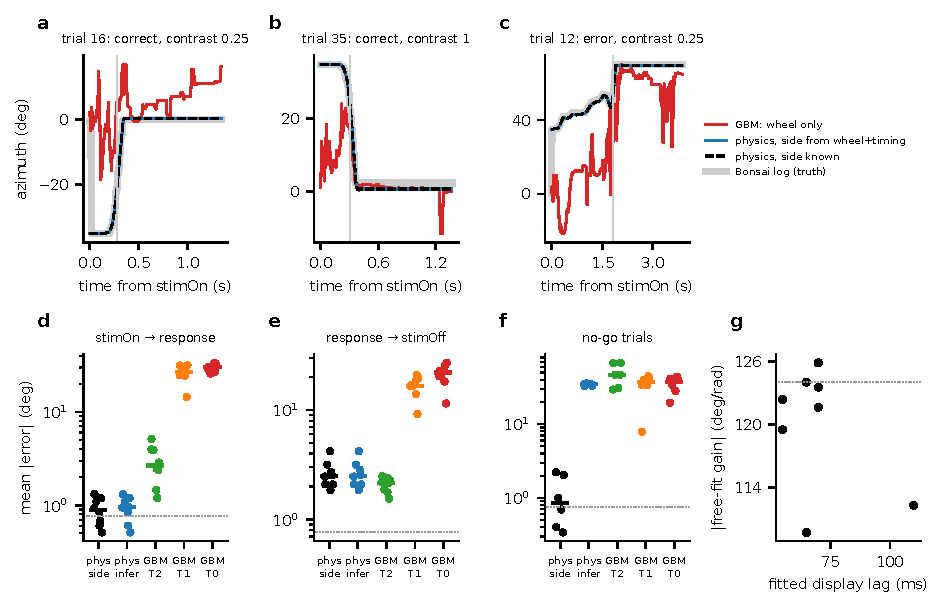
\includegraphics[width=\textwidth]{../results/fig_stim_pos_decoding.pdf}
\caption{\textbf{On-screen stimulus azimuth is recoverable from wheel position and trial timing.} Ground truth is the Bonsai stimulus-position log (\texttt{\_iblrig\_stimPositionScreen}), aligned to photodiode stimOn (residual SD 9 ms). \textbf{a--f}, Example trials chosen by per-trial $R^2$ of the physics decoder (side inferred from wheel and timing), computed over all samples from stimOn to stimOff, among the 5{,}118 answered trials of all sessions (4 trials whose logged position never moved have no $R^2$; median per-trial $R^2$ = 0.96). Panel titles give $R^2$ for the physics decoder and for the gradient-boosting (GBM) decoder given only the wheel and time since stimOn (T0), with session, trial, outcome and contrast. Left axis, stimulus azimuth: logged screen position (truth, thick grey), physics decoder $x_0 + G\,\Delta w(t-\tau)$ with $|G| = 124^\circ$/rad and displacement clipped at the $\pm35^\circ$ threshold (blue), GBM T0 (red). Right axis (purple, dashed), wheel displacement since stimOn in radians, at its own time (not shifted by the display lag). Vertical line, response time. \textbf{a, b}, Best trials: the decoder follows the truth to within an encoder step, while T0, which cannot know the starting side, has a strongly negative $R^2$. \textbf{c, d}, Trials at the median: errors come mainly from Bonsai freezing a few degrees short of the target after the response (c), which within a single trial weighs more than in the pooled score. \textbf{e, f}, Worst trials. \textbf{e}, The trials table has a corrupt stimOff time (28\,s before feedback), so the outcome, and with it the starting side, is inferred wrongly. \textbf{f}, Very fast response with the wheel already turning at stimulus onset; the logged stimulus stopped at $\approx60^\circ$ instead of the $70^\circ$ threshold. \textbf{g--i}, Mean absolute error per session (dots, $n=8$ sessions, one per lab; bars, median across sessions; log scale) for each model: physics with side known or inferred, and GBM with features T2 (wheel + all event times), T1 (wheel + response time) or T0 (wheel only), cross-validated in 5 folds grouped by trial. The dotted line marks one encoder step ($0.76^\circ$). \textbf{g}, Samples from stimOn to response on answered trials. \textbf{h}, Samples from response to stimOff on answered trials; the error of $\approx2^\circ$ comes from Bonsai freezing on the last frame before the threshold event. \textbf{i}, Samples from no-go trials (only sessions with no-go trials). Without the side, no decoder can place the stimulus. \textbf{j}, Display lag $\tau$ fitted per session against the magnitude of an unconstrained least-squares gain (dotted line: nominal 124$^\circ$/rad).}

\label{fig:main}
\end{figure}

\begin{table}[t]
\centering\small
\caption{Sessions. $\tau$, fitted display lag; $|G_\mathrm{free}|$, unconstrained gain fit (nominal
124$^\circ$/rad). The iblrig version was missing from one settings file.}
\label{tab:sessions}
\resizebox{\textwidth}{!}{\begin{tabular}{llllrrrrr}
\toprule
Session & Lab & Subject & Date & iblrig & Trials & No-go & $\tau$ (ms) & $|G_\mathrm{free}|$ \\
\midrule
\texttt{6713a4a7} & angelakilab & NYU-11 & 2020-02-18 & 6.2.5 & 565 & 9 & 70 & 123.5 \\
\texttt{034e726f} & churchlandlab & CSHL045 & 2020-02-24 & 6.2.5 & 589 & 4 & 65 & 109.7 \\
\texttt{7dd27c2f} & churchlandlab\_ucla & MFD\_05 & 2023-08-15 & -- & 525 & 1 & 55 & 122.4 \\
\texttt{0f25376f} & danlab & DY\_008 & 2020-03-03 & 6.2.5 & 471 & 1 & 70 & 125.8 \\
\texttt{64977c74} & hausserlab & PL015 & 2022-02-20 & 6.5.3 & 813 & 0 & 55 & 119.5 \\
\texttt{66d98e6e} & hoferlab & SWC\_042 & 2020-07-13 & 6.4.0 & 564 & 3 & 65 & 124.0 \\
\texttt{c4432264} & mainenlab & ZFM-01576 & 2020-12-01 & 6.4.2 & 847 & 0 & 110 & 112.3 \\
\texttt{4d8c7767} & mrsicflogellab & SWC\_038 & 2020-07-30 & 6.4.1 & 767 & 1 & 70 & 121.6 \\
\bottomrule
\end{tabular}
}
\end{table}

\section{Limitations}
\begin{itemize}
\item The lag $\tau$ is fitted on the same samples on which accuracy is reported. It is a single parameter on
$\sim10^5$ samples, so overfitting is negligible. For a new session without a position log, a fixed default of $\tau=65$\,ms costs
little. Across the 8 sessions, the mean absolute error before response rose by at most $0.2^\circ$, except in
the session with $\tau=\LagMax$\,ms (\texttt{c4432264}), where it rose from $0.84^\circ$ to $1.43^\circ$. Lags
therefore vary between rigs.
\item Only iblrig-6 sessions were tested. Newer task versions may log differently or use different settings
(gain, threshold, positions), and these should be read from \texttt{\_iblrig\_taskSettings}.
\item The side inference relies on the outcome-specific stimulus-off delays of this task version.
\item The ground truth is Bonsai's internal stimulus position, not a measurement of the rendered image. The
photodiode alignment corrects its timing, but individual frame drops are not modelled.
\end{itemize}

\section{Code}
Code: \url{https://github.com/int-brain-lab/stim_pos_from_wheel}: \texttt{load.py} (loading and clock alignment),
\texttt{decode.py} (models and metrics; \texttt{python decode.py <eids>}), \texttt{plot.py} (figure), and
\texttt{report/make\_tables.py} (tables). Build the report with \texttt{tectonic report.tex}.

\end{document}
